
\documentclass[xcolor=dvipsnames]{beamer} % dvipsnames gives more built-in colors
\usepackage[utf8]{inputenc}
\usepackage[spanish]{babel}

\mode<presentation> {

\usetheme{CambridgeUS}

%\setbeamertemplate{footline} % To remove the footer line in all slides uncomment this line
\setbeamertemplate{footline}[page number] % To replace the footer line in all slides with a simple slide count uncomment this line

\setbeamertemplate{navigation symbols}{} % To remove the navigation symbols from

\definecolor{utfsmred}{HTML}{D60019}
\definecolor{utfsmyellow}{HTML}{F7AE00}
\definecolor{utfsmgreen}{HTML}{008452}
\definecolor{utfsmblue}{HTML}{004B85}


\newenvironment<>{rosa}[1][]{
  \setbeamercolor{block title example}{fg=white,bg=blue!75!black}%
  \begin{example}#2[#1]}{
  \end{example}
}



\usecolortheme[named=utfsmblue]{structure}
\setbeamercolor{titlelike}{parent=structure,fg=utfsmblue}
\setbeamercolor{frametitle}{fg=utfsmblue}

%\setbeamercolor{section in head/foot}{bg=Brown}
%\setbeamercolor{author in head/foot}{bg=Brown}
%\setbeamercolor{date in head/foot}{fg=Brown}

\setbeamercolor*{enumerate item}{fg=utfsmred}
\setbeamercolor*{enumerate subitem}{fg=utfsmred}
\setbeamercolor*{enumerate subsubitem}{fg=utfsmred}

\setbeamercolor*{itemize item}{fg=utfsmred}
\setbeamercolor*{itemize subitem}{fg=utfsmred}
\setbeamercolor*{itemize subsubitem}{fg=utfsmred}

\setbeamercolor{item projected}{bg=utfsmred}


\setbeamertemplate{itemize items}[square]
\setbeamertemplate{enumerate items}[default]


\setbeamercolor{section in head/foot}{bg=utfsmblue}

\setbeamercolor{block title}{bg=utfsmblue!80,fg=white}
\setbeamercolor{block title alerted}{bg=utfsmred!80,fg=white}
\setbeamercolor{block title example}{bg=utfsmgreen!80,fg=white}

\setbeamertemplate{sections/subsections in toc}[square]
\setbeamercolor{section number projected}{bg=utfsmblue,fg=white}


}


\usepackage{graphicx} % Allows including images
\usepackage{booktabs} % Allows the use of \toprule, \midrule and \bottomrule in tables
\usepackage{listings}
\lstset{ %
language=C,
basicstyle=\normalsize\ttfamily,
keywordstyle=,
numbers=none,
numberstyle=\tiny\ttfamily,
stepnumber=1,
showspaces=false,
showstringspaces=false,
showtabs=false,
breaklines=true,
frame=tb,
framerule=0.5pt,
tabsize=4,
framexleftmargin=0.5em,
framexrightmargin=0.5em,
xleftmargin=0.5em,
xrightmargin=0.5em,
}

%----------------------------------------------------------------------------------------
%	TITLE PAGE
%----------------------------------------------------------------------------------------

\title{Firewalld}
\subtitle{\small{Seminario de Desarrollo de Software - Casa Central.}}
\author{Maximiliano Osorio\\\small{mosorio@inf.utfsm.cl}} 
\institute[UTFSM]
{
Universidad Técnica Federico Santa María
\medskip
}
\date{\today} % Date, can be changed to a custom date

\begin{document}
	
%-=-=-=-=-=-=-=-=-=-=-=-=-=-=-=-=-=-=-=-=-=-=-=-=
%
%	TITLE PAGE
%
%-=-=-=-=-=-=-=-=-=-=-=-=-=-=-=-=-=-=-=-=-=-=-=-=





%\begin{block}{Dependencias}
%\end{block}
\maketitle

\begin{frame}[fragile]
\frametitle{firewalld}
Firewalld es metodo por defecto de RHEL 7 para el manejo de firewall.


\begin{itemize}
\item Es dinamico porque las reglas se aplican de forma inmediata y sin necesidad de reinicio.
\item Soporta IPv4 y IPv6.
\item Utiliza iptables (tool) para comunicar con el kernel (netfilter)
\end{itemize}

\end{frame}


\begin{frame}{Firewalld}
	\begin{figure}
		\centering
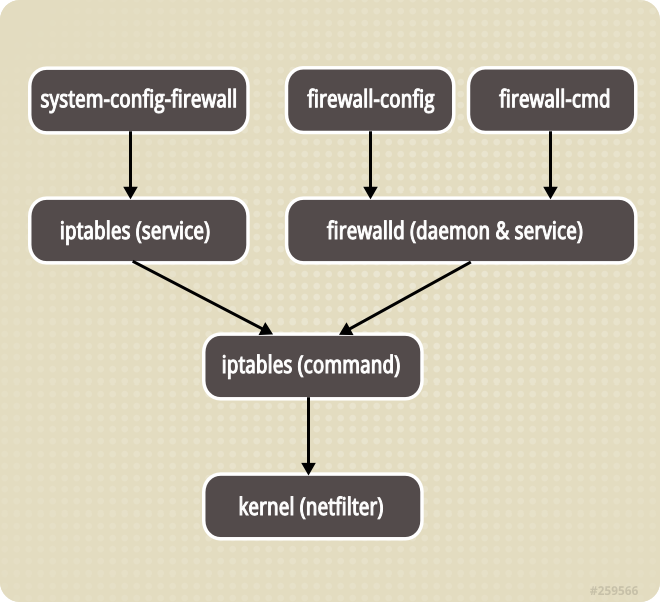
\includegraphics[width=\textwidth,height=0.8\textheight,keepaspectratio]{images/firewall_stack}
    \end{figure}
\end{frame}


\begin{frame}[fragile]
\frametitle{Zones}
firewalld separa todo el \textit{incoming traffic} por red en zonas, cada zona tiene un set de reglas.


\begin{itemize}
\item \textbf{drop}
 Any incoming network packets are dropped, there is no reply. Only outgoing network connections are possible.
\item \textbf{block}
Any incoming network connections are rejected with an icmp-host-prohibited message for IPv4 and icmp6-adm-prohibited for IPv6. Only network connections initiated from within the system are possible.
\item \textbf{public}
For use in public areas. You do not trust the other computers on the network to not harm your computer. Only selected incoming connections are accepted.
\item \textbf{external}
For use on external networks with masquerading enabled especially for routers. You do not trust the other computers on the network to not harm your computer. Only selected incoming connections are accepted.

\end{itemize}
\end{frame}

\begin{frame}[fragile]
\frametitle{Zonas}
\begin{itemize}

\item \textbf{dmz}

For computers in your demilitarized zone that are publicly-accessible with limited access to your internal network. Only selected incoming connections are accepted.
\item \textbf{work}
For use in work areas. You mostly trust the other computers on networks to not harm your computer. Only selected incoming connections are accepted.
\item \textbf{home}

For use in home areas. You mostly trust the other computers on networks to not harm your computer. Only selected incoming connections are accepted.
\item \textbf{internal}
For use on internal networks. You mostly trust the other computers on the networks to not harm your computer. Only selected incoming connections are accepted.
\item \textbf{trusted}
All network connections are accepted.
\end{itemize}
\end{frame}


\begin{frame}[fragile]
\frametitle{Servicios}
Existen servicios ya definidos
\begin{lstlisting}
~]# ls /usr/lib/firewalld/services/
\end{lstlisting}


\begin{lstlisting}
firewall-cmd --get-services
RH-Satellite-6 amanda-client bacula bacula-client dhcp dhcpv6 dhcpv6-client dns ftp high-availability http https imaps ipp ipp-client ipsec kerberos kpasswd ldap ldaps libvirt libvirt-tls mdns mountd ms-wbt mysql nfs ntp openvpn pmcd pmproxy pmwebapi pmwebapis pop3s postgresql proxy-dhcp radius rpc-bind samba samba-client smtp ssh telnet tftp tftp-client transmission-client vnc-server wbem-https
\end{lstlisting}


\end{frame}

\begin{frame}[fragile]
\frametitle{Quickstart}
\begin{lstlisting}
~]# yum -y install firewalld
~]# systemctl stop firewalld
~]# systemctl disable firewalld
~]# systemctl start firewalld
~]# systemctl enable firewalld
\end{lstlisting}


\end{frame}


\begin{frame}[fragile]
\frametitle{Status}
\begin{lstlisting}
~]# systemctl status firewalld
~]$ firewall-cmd --state
running
\end{lstlisting}

\begin{lstlisting}
~]$ firewall-cmd --state
running
\end{lstlisting}
\end{frame}

\begin{frame}[fragile]
\frametitle{Zonas}
Añadir un interfaz a una zona.
\begin{lstlisting}
~]# firewall-cmd --zone=public --add-interface=em1
\end{lstlisting}
\end{frame}

\begin{frame}[fragile]
\frametitle{Zonas}
Mostrar las zonas activas
\begin{lstlisting}
~]$ firewall-cmd --get-active-zones
public
  interfaces: em1
\end{lstlisting}
\end{frame}

\begin{frame}[fragile]
\frametitle{Zonas}
Mostrar la zona de una interfaz
\begin{lstlisting}
~]$ firewall-cmd --get-zone-of-interface=em1
public
\end{lstlisting}
\end{frame}

\begin{frame}[fragile]
\frametitle{Zonas}
Listas las interfaces en una zona
\begin{lstlisting}
~]# firewall-cmd --zone=public --list-interfaces
em1 wlan0
\end{lstlisting}
\end{frame}



\begin{frame}[fragile]
\frametitle{Listar}
\begin{lstlisting}
firewall-cmd --zone=public --list-ports
firewall-cmd --zone=public --list-services
\end{lstlisting}
\end{frame}

\begin{frame}[fragile]
\frametitle{Zonas}
Listar servicios y puertos en una zona
\begin{lstlisting}
~]# firewall-cmd --zone=public --list-all
public
  interfaces: 
  services: mdns dhcpv6-client ssh
  ports: 
  forward-ports: 
  icmp-blocks: source-quench
\end{lstlisting}
\end{frame}



\begin{frame}[fragile]
\frametitle{Servicios}
Listar servicios
\begin{lstlisting}
~]# firewall-cmd --permanent --get-services
\end{lstlisting}
\end{frame}

\begin{frame}[fragile]
\frametitle{Añadir un puerto}
\begin{lstlisting}
~]# firewall-cmd --zone=dmz --add-port=8080/tcp
~]# firewall-cmd --zone=public --add-port=5060-5061/udp
\end{lstlisting}

\end{frame}



\begin{frame}[fragile]
\frametitle{Añadir un servicio}
\begin{lstlisting}
~]# firewall-cmd --zone=work --add-service=smtp
\end{lstlisting}
\end{frame}


\begin{frame}[fragile]
\frametitle{Remueve un servicio}
\begin{lstlisting}
~]# firewall-cmd --zone=work --remove-service=smtp
\end{lstlisting}


\end{frame}


\begin{frame}[fragile]
\frametitle{Permanent}
Si quiere que la regla se mantenga después de un reboot, se añade \textbf{ --permanent} y es \textbf{necesario} el reload
\begin{lstlisting}
~]# firewall-cmd --permanent --zone=work --remove-service=smtp
~]# firewall-cmd --reload
\end{lstlisting}
Esto no rompera las conexiones establecidas, si desea hacer eso debe utiliza \textbf{--complete-reload}, que va a cortar todas las conexiones establecidas.

\end{frame}


\begin{frame}[fragile]
\frametitle{Añadir un puerto para ciertos destino}

172.25.1.0/24: representa a red de los hosts 172.25.1.0-255.

\begin{lstlisting}
~]# firewall-cmd --zone=work --add-port=8080/tcp --add-source 172.25.X.0/24
\end{lstlisting}
\end{frame}



\begin{frame}[fragile]
\frametitle{Rich rules}
Con el \textit{rich languague}, se pueden crear reglas complejas en una forma sencilla utilizando zonas. 

\begin{lstlisting}
firewall-cmd [--zone=zone] --add-rich-rule='rule' [--timeout=seconds]
firewall-cmd [--zone=zone] --query-rich-rule='rule'
firewall-cmd [--zone=zone] --remove-rich-rule='rule'

\end{lstlisting}
\end{frame}
\begin{frame}[fragile]
\frametitle{rich rules}
\begin{lstlisting}
rule [family="rule family"]
    [ source address="address" [invert="True"] ]
    [ destination address="address" [invert="True"] ]
    [ element ]
    [ log [prefix="prefix text"] [level="log level"] [limit value="rate/duration"] ]
    [ audit ]
    [ action ]
    
\end{lstlisting}
%\href{https://access.redhat.com/documentation/en-US/Red_Hat_Enterprise_Linux/7/html/Security_Guide/sec-Using_Firewalls.html#sec-Configuring_firewalld{Mas información}
\end{frame}


\begin{frame}[fragile]
\frametitle{rich rules}
\begin{lstlisting}
firewall-cmd  --add-rich-rule='rule family=ipv4 source address=10.10.15.123/32 reject'
firewall-cmd  --add-rich-rule='rule family=ipv4 source address=10.10.15.123/32 drop'
firewall-cmd  --add-rich-rule='rule service name="ssh" log prefix="SSH PRUEBA!!" level="notice" accept'
firewall-cmd  --add-rich-rule='rule  to-port="80" log prefix="HTTP PRUEBA!!" level="notice" log limit value="1/m" accept'
\end{lstlisting}

\end{frame}

\begin{frame}[fragile]
\frametitle{direct rules}
\begin{lstlisting}
# firewall-cmd --permanent --direct --add-rule ipv4 filter OUTPUT 0 -p tcp -m tcp --dport=22 -j ACCEPT
success
# firewall-cmd --permanent --direct --add-rule ipv4 filter OUTPUT 1 -p tcp -m tcp --sport=22 -j ACCEPT
success
# firewall-cmd --permanent --direct --add-rule ipv4 filter OUTPUT 9 -j DROP
success
\end{lstlisting}

\end{frame}

\end{document}


